\documentclass[12pt]{article}

\usepackage{
    amssymb,
    amsmath,
    amsfonts,
    eurosym,
    geometry,
    ulem,
    graphicx,
    caption,
    color,
    setspace,
    sectsty,
    comment,
    footmisc,
    caption,
    natbib,
    pdflscape,
    subfigure,
    array,
    hyperref,
    booktabs,
    longtable,
    float,
    threeparttable}
% \usepackage[
%     backend=biber,
%     style=nature,
%     doi=false,
%     isbn=false,
%     url=false,
%     eprint=false
%     ]{biblatex}
        

\normalem

\onehalfspacing
\newtheorem{theorem}{Theorem}
\newtheorem{corollary}[theorem]{Corollary}
\newtheorem{proposition}{Proposition}
\newenvironment{proof}[1][Proof]{\noindent\textbf{#1.} }{\ \rule{0.5em}{0.5em}}

\newtheorem{hyp}{Hypothesis}
\newtheorem{subhyp}{Hypothesis}[hyp]
\renewcommand{\thesubhyp}{\thehyp\alph{subhyp}}

\newcommand{\red}[1]{{\color{red} #1}}
\newcommand{\blue}[1]{{\color{blue} #1}}

\newcolumntype{L}[1]{>{\raggedright\let\newline\\arraybackslash\hspace{0pt}}m{#1}}
\newcolumntype{C}[1]{>{\centering\let\newline\\arraybackslash\hspace{0pt}}m{#1}}
\newcolumntype{R}[1]{>{\raggedleft\let\newline\\arraybackslash\hspace{0pt}}m{#1}}

\geometry{left=1.0in,right=1.0in,top=1.0in,bottom=1.0in}

\addbibresource{lipids.bib}

\begin{document}

\begin{titlepage}
\title{Long-term and recent trends in serum cholesterol treatment and control in 14 high-income countries: an analysis of 1XX nationally representative surveys}
\author{NCD Risk Factor Collaboration (NCD-RisC)\thanks{Full author list at end of the article}}
\date{\today}
\maketitle

\end{titlepage}
\emptythanks
\clearpage
\begin{abstract}
    \noindent \textbf{Background:} Lipid-lowering therapies are effective at preventing cardiovascular events and are therefore recommended by national and international guidelines. However, guidelines are not uniform nor are they consistently applied across countries. We aim to compare treatment and control of elevated serum cholesterol in high-income countries over time.
    \vspace{0.5em} \\
    \noindent \textbf{Methods:} We used data from people aged 40-79 years who participated in 1XX nationally representative health examination surveys from 1990 to 2020 in 14 high-income countries: Australia, Belgium, Chile, the Czech Republic, Finland, Ireland, Italy, Malta, Poland, Slovakia, South Korea, Spain, the UK, and the USA. Accounting for complex survey design, we calculated the proportion of participants eligible for lipid-lowering therapy, which was defined as non-HDL-C 5.69 mmol/L (220 mg/dL) or more, or a combination of elevated 10-year risk of cardiovascular disease and non-HDL-C levels above guideline, or being on pharmacological treatment for elevated serum cholesterol. We also calculated the proportion of those eligible who were treated and whose serum cholesterol levels were optimally controlled (i.e. non-HDL-C lower than 3.36 mmol/L or 130 mg/dL).
    \vspace{0.5em} \\
    \noindent \textbf{Findings:} Data from XXX XXX participants met our inclusion criteria. The prevalence of elevated serum cholesterol varied substantially and declined over time in all countries except South Korea and Poland. In the early 1990s, treatment coverage was close to zero, but increased rapidly after 2000. Improvements occurred first in the USA and Australia with coverage in most other countries only converging after 2010. In their most recent surveys, South Korea, the UK, and the USA had the highest rates of treatment and control, whereas Finland, Slovakia, and Italy had the lowest. Despite progress, treatment coverage was still less than 80\% and optimal control was less than 60\% in the best performing countries. Treatment coverage declined with age in all countries, even in high risk subgroups. Among 40-49 year olds with elevated serum cholesterol, the prevalence of untreated severe ($>$ 5.69 mmol/L non-HDL-C) hypercholesterolemia was between 20 and 40\%.
    \vspace{0.5em} \\
    \noindent \textbf{Interpretation:} Treatment and control of elevated serum cholesterol have improved substantially in high-income countries since the 1990s. However, few countries have achieved rates of optimal treatment and control of high-quality hypercholesterolemia programmes. Considerable gaps remain in treatment coverage among younger age groups at high risk. 
    \vspace{1em} \\
    \noindent\textbf{Keywords:}  cholesterol, hypercholessterolemia therapy, statins, hypercholesterolemia epidemiology \vspace{0.5em} \\
    \noindent\textbf{Word count:} 3,950
    \end{abstract}
    \setcounter{page}{0}
    \thispagestyle{empty}
\doublespacing

\begin{refsection}
\section{Introduction} \label{sec:introduction}
Elevated serum cholesterol, particularly in the form of non high-density lipoproteins (non-HDL-C), is a major risk factor for the development of atherosclerosis and subsequent coronary heart disease or ischaemic stroke \cite{prospective_studies_collaboration_blood_2007,law_by_1994}. Lipid-lowering therapies, such as statins, can lower serum cholesterol level and reduce the risk of cardiovascular disease \cite{cholesterol_treatment_trialists_ctt_collaboration_efficacy_2005,cholesterol_treatment_trialists_ctt_collaboration_efficacy_2010}. Most national guidelines now recommend pharmacological treatment even among patients with moderately elevated serum cholesterol levels provided they meet certain risk criteria \cite{grundy_scott_m_2018_2019,mach_2019_2020,rabar_lipid_2014,kinoshita_japan_2018,rhee_2018_2019,national_heart_foundation_of_australia_and_the_cardiac_society_of_australia_and_new_zealand_position_2005} based on randomized clinical trial evidence demonstrating efficacy of reducing cholesterol for primary prevention of cardiovascular disease \cite{cholesterol_treatment_trialists_ctt_collaborators_effects_2012}. For instance, the major cardiology associations in both the United States \cite{grundy_scott_m_2018_2019} and Europe \cite{mach_2019_2020} now recommend treatment among those with low-density lipoprotein cholesterol (LDL-C) $>$ 70 mg/dL (non-HDL-C $>$ 100 mg/dL) if they have moderate risk factor levels. Yet, debates about the risk and benefits of preventative therapy, particularly in low risk populations, continued for years and led, for a time at least, to considerable heterogeneity in guidance about the treatment of cholesterol across countries \cite{smith_should_1992,abramson_should_2013}. 

However, despite the availability of lipid-lowering drugs and mass publicization of treatment guidelines, there are few comparative multi-country studies contrasting countries in terms of treatment and control of serum cholesterol \cite{roth_high_2011,marcus_use_2022,taddei_repositioning_2020-1}. This is true even among high-income countries where health systems have more resources and the barriers to access are fewer. In this study, we use data from nationally representative health examination surveys to benchmark the performance on control and treatment of serum cholesterol across 1X high-income countries, with different health systems and treatment approaches, over a period of three decades coinciding with the authorization and wide distribution of statins. 

\section{Methods} \label{sec:methods}
\subsection{Data sources}
In this study, we used data from 1XX nationally representative health examination surveys completed between 1990 and 2020 in 14 countries: Australia, Belgium, Chile, the Czech Republic, Finland, Ireland, Italy, Malta, Poland, Slovakia, South Korea, Spain, the United Kingdom, and the United States of America. These surveys included a lipid panel for a random sample of the general population as well as questions about lipid-lowering treatment. We chose 1990 as our baseline to coincide with the initial wave of regulatory approvals for statins \cite{tobert_lovastatin_2003}. A complete list of surveys and information about their design, including the age range and number of participants as well as the devices used, is included in Table \ref{tab:data_sources}. Countries were defined as ``high-income'' based on the 2020 World Bank classification.

We include data from men and women between 40-79 years of age, as this population is the focus of national cholesterol treatment guidelines for primary and secondary prevention. We did not include participants under 40 years of age as pharmacological treatment in this group is rare, and did not include participants over 80 years of age as guidelines and therapeutic goals for primary prevention are different. All analyses are stratified by sex and age categorized in 10-year groups. We therefore excluded 7,161 participants (2.5\%) from surveys in which we had less than 5 years from a particular age group. Participants with missing data on serum cholesterol levels, treatment, or other risk factors necessary to calculate risk score were also excluded from the analysis (X\%). After exclusion, we had data on XXX XXX participants (see Appendix Figure \ref{fig:exclusion}).

\subsection{Outcomes}
We defined elevated serum cholesterol as non-HDL-C of 5.69 mmol/L or more, or non-HDL-C of 4.91 mmol/L or more and 10-year risk of CVD greater than 5\%, or non-HDL-C of 4.14 mmol/L or more and 10-year risk greater than 10\%, or non-HDL-C of 3.36 mmol/L or more and 10-year risk greater than 20\%, or being on pharmacological treatment with lipid-lowering drugs (see Box \ref{box:first}). We used non-HDL-C levels, defined as total serum cholesterol level minus HDL-C, to determine eligibility, rather than LDL-C because direct measurements of LDL-C were not available in many surveys and the alternative, to calculate it via the Friedewald equation, requires data on triglycerides and can be inaccurate. There may also be physiological reasons to prefer non-HDL-C as a measure of atherosclerotic risk \cite{packard_non-hdl_2004,blaha_importance_2008,ridker_nonhdl_2005, ncd_risk_factor_collaboration_ncd-risc_national_2020-1} as it also includes lipoprotein(a), intermediate-density lipoprotein, very-low-density lipoprotein and lipoprotein remnants. Among surveys measuring both, non-HDL-C and LDL-C were highly correlated (see Appendix Figure \ref{fig:callibration} and ref \cite{ncd_risk_factor_collaboration_ncd-risc_national_2020-1}). When converting LDL-C cut-offs in treatment guidelines to non-HDL-C levels we added 0.78 mmol/L (30 mg/dL) as suggested by several sources \cite{noauthor_third_2002,mach_2019_2020}. National guidelines for cholesterol therapy differ across countries (see Appendix Table \ref{tab:guidelines}), in the main text we used the unified definition in Box \ref{box:first} to increase comparability, however in the Appendix we also present estimates based on country-specific guidelines (see Appendix Table \ref{tab:sensitivity_national}). For risk-based thresholds, we used country and year-specific predicted risk estimates for 10-year cumulative incidence of cardiovascular disease based on \textit{Globorisk} \cite{hajifathalian_novel_2015,ueda_laboratory-based_2017}, a country-year recalibrated risk score based on multiple cohorts and recalibrated for each country's CVD and risk factor profile in each year (see Appendix \ref{sec:risk_scores}). In many guidelines, those diagnosed with diabetes mellitus are considered treatment eligible regardless of their serum cholesterol levels or at only moderately elevated levels. In the appendix, we present estimates that modify our eligibility criteria to include anyone diagnosed with diabetes (Appendix Table \ref{tab:sensitivity_national}). 

We established whether participants had been pharmacologically treated for elevated serum cholesterol using survey-specific questions, which were typically worded in the following way: ``Because of your high cholesterol, have you ever been told to take prescribed medicine? Are you now taking it?'' and ``Are you currently taking any medicines, tablets or pills for high cholesterol?'' We took a similar approach in surveys that had gathered information on medicines prescribed to the participants, by relying on survey information about elevated serum cholesterol being the purpose or diagnosis leading to taking a lipid-lowering medicine. In surveys in which these questios were followed up with further verification of the type of medication, more than 90\% were statins.

The optimal serum cholesterol level as a target for treatment has shifted over time and is still subject to debate \cite{grundy_statin_1998,deedwania_reduction_2006}. We defined participants with pharmacologically controlled serum cholesterol levels as those on treatment who had attained non-HDL-C levels below 3.36 mmol/L as this seems to be the consensus target set in a majority of countries \cite{mach_2019_2020,grundy_scott_m_2018_2019,rhee_2018_2019}. However, in the appendix, we also present results at other thresholds (see Appendix Table \ref{tab:control_sensitivity}).

Immediate treatment is recommended for people with severe hypercholesterolemia (i.e. non-HDL-C greater than 5.69 mmol/L) by all guidelines and failure to provide treatment in such cases is a sign of the inadequate performance of the health-care system. Hence, we also examine the proportion of people with untreated severe hypercholesterolemia across country age and sex groups.

\subsection{Statistical analysis}
In each survey, we calculated mean non-HDL-C levels and the prevalence of elevated serum cholesterol levels and their 95\% CIs overall and stratified by sex and age. We also calculated the proportion with elevated serum cholesterol levels who reported using lipid-lowering medication (treatment) and the proportion with elevated serum cholesterol levels who were on treatment and had non-HDL-C levels below 3.36 mmol/L (controlled). Finally, we calculate the proportion with elevated serum cholesterol who were untreated and had non-HDL-C levels above 5.69 mmol/L (severe hypercholesterolemia). We accounted for complex survey design and used survey sample weights when calculating prevalence, treatment, and control. We estimated standard errors for all proportions using the method of Korn and Graubard \cite{korn_confidence_1998} to account for clustering where applicable. All analyses were conducted using R version 4.3 and the \texttt{survey} package.

\section{Results} \label{sec:result}

\subsubsection*{Long-term trends in prevalence, treatment, and control}
Mean serum non-HDL-C levels declined by an average of 0.31 mmol/L per decade across all countries between 1990 and 2020, ranging from 0.45 mmol/L per decade in the UK to 0.12 mmol/L per decaed in South Korea. Levels declined similarly for men andwomen, but declines were generally larger for older age groups than younger age groups (figure \ref{fig:mean_chol}). In terms of lipid fractions, the observed decrease in mean serum non-HDL-C  a decline in total serum cholesterol levels across all countries while serum HDL-C levels increased modestly (figures \ref{fig:tc} to \ref{fig:ldl}).

Likewise, the prevalence of elevated serum cholesterol requiring treatment declined by an average of 5.6 percentage points per decade between 1990 and 2020 (figure \ref{fig:eligible}), driven by the aforementioned decreases in non-HDL-C levels as well as secular changes in cardiovascular risk and declines in prevalence of smoking (figure \ref{fig:smoker}). A notable exception was South Korea where prevalence of elevated serum cholesterol increased by about 8.1 percentage points per decade between 1990 and 2020, with similar trends within sex and age groups. However, it should be noted South Korea also started from a much lower baseline prevalence in 2005 and the increase mostly translated into convergence in prevalence of elevated cholesterol with its peers by 2020. There were strong age and sex gradients in trends in prevalence of elevated serum cholesterol over time. Prevalence generally declined more among older age groups than younger age groups and more among women than men.

Treatment of elevated serum cholesterol increased dramatically in all countries (figure \ref{fig:treated}) with improvements in most places accelerating after the year 2000. Pooling across all age and sex groups treatment coverage among those eligible increased by an average of 3.1 percentage points per year between 1990 and 2020. Within age and sex groups, improvements in treatment coverage were generally higher amongst those 60-79 years of age and lowest amongst those 40-59 years of age. Increases in coverage were generally higher for women at young ages and higher for men at older ages. Looking population-wide, rather than just among those eligibile, we observed similar trends in treatment coverage (figure \ref{fig:treated_pop}).

Trends in the proportion of people with elevated serum cholesterol on treatment whose cholesterol levels were controlled (i.e. achieved non-HDL-C levels of 2.98 mmol/L or lower) followed a similar trajectory to trends in lipid-lowering treatment, but at a lower level. Across all countries the proprotion controlled increased by an average of 2.7 percentage points per year, starting near zero around 2000 and reaching 60-70\% by 2020 in some country age and sex groups, such as in men and women over 60 in the United Kingdom. However, overall proportions remain below 50\% at most recent survey in most countries. As with treatment, increases in the control of serum cholesterol were steeper among older age groups than younger age groups. 

\subsubsection*{Variation in timing of treatment adoption across countries}

Improvements in treatment coverage occurred first in the USA and Australia in the early 2000s, but some countries caught up by the late 2010s (figure \ref{fig:treated}). For instance, in 2005 coverage was 57\% in Australia and 51\% in the USA as compared just 36\% in the United Kingdom. Looking within age and sex strata, this early lead in treatment adoption in the USA and Australia occurred mostly among those over 60 years of age. Their lead also persisted when examining treatment coverage in the full 40-79 population (figure \ref{fig:treated_pop}), rather than among those eligible, nor was there a discernable difference in the prevalence of eligibility suggesting variation was not due simply to shifting diagnosis patterns. 

Outside the USA and Australia, most countries saw progress in treatment coverage only after the mid 2000s, with the most rapid changes happening after 2010. Amongst later adopters, most notable is the experience of the UK where treatment coverage at most age and sex groups lagged significantly behind those in the US and Australia throughout the 2000s, but by the second half of the 2010s coverage in the UK had caught up and even surpassed them (2018 USA: 74\%, UK: 77\%). Indeed, between 2010 and 2018 treatment coverage improved by 35 percentage points in the UK, from 42\% to 77\%, compared to an increase of only 14 percentage points in the USA over the same time period.

While treatment coverage has mostly converged among younger age groups, in older age groups and especially among men, South Korea and Chile lag significantly behind their peer countries. As shown in Figure 5, the lead in treatment coverage amongst early adopters also did not always translate to advantages in the proportion controlled, particularly in the USA. In the 2000s, when their lead in treatment coverage was greatest, the USA's lead in control was about half as high (Australia: 33\%, USA: 23\%, UK: 18\%). 

\subsubsection*{Recent trends and remaining gaps in treatment coverage and control}

In the most recent national surveys, the prevalence of elevated serum cholesterol was highest in Poland (50\%) and lowest in Finland (17\%) and Chile (20\%) (figure \ref{fig:recent}). Treatment was highest in the UK (82\%), Poland (77\%), and US (74\%), and lowest in Finland (31\%). Control was highest in the UK (66\%), South Korea (54\%), and Australia (51\%), and lowest in Finland (8\%). Within age and sex strata, prevalence was higher among older age groups and among men. Treatment and control were also generally higher among older age groups with older men more likely to be treated and to have controlled serum cholesterol than older women. However,  the reverse was generally true in younger age groups, i.e. treatment and control were higher among younger women than younger men. 

There were notable gaps in treatment coverage among younger participants with elevated serum cholesterol across all countries. In recent surveys, treatment coverage was between 40 and 50\% in most countries among those eligible and  40-49 years of age compared to 70 to 80\% among those eligible and 60-79 years of age (figure \ref{fig:gaps}). Indeed, despite constituting a minority of cases of elevated serum cholesterol overall, the youngest age groups had persistently high unmet need amongst those at highest risk, defined as those with untreated severe hypercholesterolemia (i.e. non-HDL-C $>$ 5.69 mmol/L). The proportion with untreated severe hypercholesterolemia ranged from 20\% to 40\% in 40-49 year olds as compared to less than 5\% in older age groups. 
%Untreated severe hypercholesterolemia was highest in X and lowest in Y.

There were also gaps in the proportion with controlled serum cholesterol levels as compared to those on treatment in some countries (figure \ref{fig:recent}). For instance, in Poland there was a 40 percentage point gap in the proportion on treatment and the proportion with controlled serum cholesterol levels for both men and women. 


\section{Discussion} \label{sec:discussion}
Using data from more than X participants in 1XX national health examination surveys from 1X high-income countries, we found that treatment and control of elevated serum cholesterol has improved dramatically in all countries since at least 2000, accompanied by declines in prevalence of elevated serum cholesterol and in mean non-HDL-C levels. However, optimal control rates remain below 50\% in most countries. This is significantly lower than the rates achieved by regional high-quality cholesterol treatment and education programmes\cite{koren_clinical_2004}. Suboptimal control can occur when those with elevated serum cholesterol are not diagnosed and treated but also when those who are treated fail to achieve the necessary reductions in serum cholesterol levels, because of poor adherence, insufficient dosing, or nonresponse. In our sample, between X\% and Y\% fall into the latter category. 

Prior multinational studies comparing trends in serum cholesterol treatment and control in high-income countries, to our knowledge, are exceedingly rare. One study in 8 high- and middle-income countries charted an increase in treatment in US and UK between 1998 and 2007 but didn't examine variation within high-income countries in depth, focusing instead on differences between high- and middle-income countries \cite{roth_high_2011}. A more recent analysis \cite{marcus_use_2022} in low- and middle-income countries between 2007 and 2018 found significant variation in treatment and control rates between countries, but at a much lower level (less than 30\% and 7\%, respectively) than observed among high-income countries in our study and was not able to investigate trends in performance over time. Changes in treatment and control rates over time have primarily been reported in individual countries \cite{muntner_trends_2013}. Most noted the rapid increase in treatment in the early 2000s, but did not benchmark this progress against peer nations. Only a handful of published studies in individual countries document trends in the 2010s as treatment guidelines consolidated and risk thesholds and cholesterol targets were progressively lowered.

The strengths of our study include nearly three decades of high-quality and consistently cleaned comparative data from nationally representative survey samples across 14 countries, which allows us to track trends and variation across countries. We are also able to identify those eligibile for risk-based treatment using country-specific predicted CVD risks from \textit{Globorisk}. A limitation is that few studies were available prior to late 1990s and early 2000s, restricting comparisons during this period; however treatment options, guidelines, and availability during this period were also different than post 2000. Another limitation is that most surveys did not record whether participants had been diagnosed with CVD prior to starting therapy, preventing us from separating out trends in primary versus secondary prevention. Similarly, many surveys did not adequately track participant's awareness of their elevated serum cholesterol levels, preventing us from separating failure to diagnose from failure to adhere to treatment. The questions about pharmacological treatment in most national health examination surveys did not distinguish between statins and other lipid-lowering drugs, although evidence from those that did suggests statins form the vast majority. A lack of data also limits our ability to track dosage or intensity of statin or whether it was prescribed as part of a combination therapy. 

The increase in treatment and control of serum cholesterol in the 2000s was likely due to the more widespread uptake of and compliance with, clinical guidelines for treatment of cholesterol, such as those put out by the National Cholesterol Education Program (NCEP) in the United States (see Appendix table \ref{tab:guidelines} for details on national and international guidelines). Thresholds for treatment have trended progressively lower over the study period and may have contributed to increasing treatment and control among those at lower risk for cardiovascular disease. Over time, newer classes of lipid-lowering drugs, including statins \cite{cholesterol_treatment_trialists_ctt_collaboration_efficacy_2010}, ezetimibe \cite{cannon_ezetimibe_2015}, and PCSK9 inhibitors \cite{sabatine_evolocumab_2017,schwartz_alirocumab_2018}, as well as more aggressive dosing regimens may have improved treatment efficacy and therefore control for some patients, although several have received full regulatory approval only. Additionally, increasing use of combination therapies (e.g. statins plus ezetimibe or statins plus PCSK9 inhibitor) may have helped those with persistently high serum cholesterol levels achieve more ambitious reduction targets.

While the prevalence of untreated severe hypercholesterolemia was generally low amongst older age groups, we noted higher burdens amongst younger age groups. Despite recommendations from national guidelines \cite{piepoli_2016_2016,de_backer_european_2003,mach_2019_2020,grundy_scott_m_2018_2019,stone_2013_2014,noauthor_third_2002,kinoshita_japan_2018,rhee_2018_2019,rabar_lipid_2014}, this may reflect lower acceptance among providers and patients for pharmacological interventions at younger ages as well as gaps in screening for hypercholesterolemia among these age groups, who often have less frequent contact with primary care clinicians. This is important as early detection and treatment of severe hypercholesterolemia in younger age groups can prevent subsequent morbidity and mortality.

We also noted large gaps in treatment and control of serum cholesterol across countries. While the challenges of getting people with elevated serum cholesterol levels on treatment are well-known, including proper screening and routine primary care, this gap may reflect the fact that the challenges of proper dosing, continuing adherence, and financial and health system support are even more substantial. 

Heterogeneity in treatment and control across countries might be partly related to differences in guidance to clinicians regarding pharmacological treatment. For example, throughout the early 2000s, guidelines outside of the United States were consistently more conservative in their approach to treatment, either stipulating higher cholesterol and risk thresholds, or the need for a period of lifestyle interventions prior to initiation of drug therapy. In European guidelines \cite{pyorala_prevention_1994,wood_prevention_1998,de_backer_european_2003,graham_european_2007}, pharmacological treatment of even those with prior CVD was not recommended until 2010. In the UK, guidelines \cite{shepherd_strategies_1987,betteridge_management_1993,society_joint_1998,society_jbs_2005} recommended  treatment only for those at very high 10-year risk of CVD ($>$20\%) until 2014. In Japan and South Korea, dietary interventions were recommended as first line treatment regardless of risk until 2012 and 2015 respectively. By contrast, in the US pharmacological treatment was recommended for intermediate risk groups earlier. Notably, both the 2004 NCEP ATP III \cite{noauthor_third_2002} and 2013 ACC/AHA guidelines \cite{stone_2013_2014} in the US set ambitious cholesterol treatment and reduction targets. Guidelines also differed in the extent that they relied on predicted cardiovascular risk versus serum cholesterol measurements plus counting of risk factors in determination of treatment eligibility. This might also contribute to the observed variation in treatment across countries. In particular, South Korea, which had below average treatment coverage among those over 70, does not include an assessment of predicted risk cardiovascular risk when determining treatment eligibility.

Beyond guidelines, health system characteristics that facilitate or impede contact with providers, including insurance, co-payment for physician consultation or prescription, and pay-for-performance incentives to physicians, might affect how often people see their physicians and have their cholesterol measured, whether lipid-lowering medicines are prescribed, and whether patients comply with the treatment (see appendix pp X for information on health systems in these 1X countries). Differences in availability of drugs may also play a role, such as the decision by the Department of Health in the UK that low-dose statins could be sold over the counter \cite{lancet_otc_2004} in 2004, or the wider availability of generics after inclusion of statins in the WHO Essential Medicines List \cite{kishore_modernizing_2018}. In addition to these systems determinants, differences in the tone and frequency of media coverage of statins across countries may further affect adherence and initiation \cite{matthews_impact_2016}. Overall, the countries with the best cholesterol control—ie, the USA, South Korea, and the UK—all have national programmes for cholesterol education or health check-up (Appendix pp 25-28). 

Dozens of randomised trials have shown the benefits of treating elevated serum cholesterol, at progressively lower risk thresholds \cite{cholesterol_treatment_trialists_ctt_collaborators_effects_2012} and with more ambitious cholesterol reduction targets \cite{cholesterol_treatment_trialists_ctt_collaboration_efficacy_2005,cholesterol_treatment_trialists_ctt_collaborators_effects_2012}. Our results show that when incorporated in guidelines and implemented in effective health systems, treatment coverage and control can rapidly increase. Yet even in these well-resourced countries, coverage and control vary substantially across countries, and rarely reach the levels achieved in high-quality regional cholesterol programmes. Increasing diagnosis and treatment, however, requires mechanisms and incentives that increase contact with health-care systems \cite{asch_effect_2015}, especially for disadvantaged groups that typically have higher prevalence of hypercholesterolemia, high CVD risk,  and lower rates of diagnosis and treatment. National health systems should set ambitious targets, and experiment and rigorously evaluate innovative mechanisms at the facility and community levels to improve cholesterol awareness, treatment, and control. Doing so would help to address the large burden of atherosclerosis and cardiovascular disease.


\singlespacing

\clearpage

\onehalfspacing

\clearpage

% \section*{Figures} \label{sec:fig}
% \addcontentsline{toc}{section}{Figures}

\begin{mybox}[floatplacement=p,label={box:first}]{Definition of elevated serum cholesterol requiring treatment}
non-HDL-C levels:
    \begin{itemize}
        \item non-HDL-C $>$ 5.69 mmol/L (220 mg/dL)
        \item non-HDL-C $>$ 4.92 mmol/L (190 mg/dL) and risk $>$5\% 
        \item non-HDL-C $>$ 4.14 mmol/L (160 mg/dL) and risk $>$10\%
        \item non-HDL-C $>$ 3.36 mmol/L (130 mg/dL) and risk $>$20\%
    \end{itemize}

LDL-C levels:
    \begin{itemize}
        \item LDL-C $>$ 4.92 mmol/L (190 mg/dL)
        \item LDL-C $>$ 4.14 mmol/L (160 mg/dL) and risk $>$5\% 
        \item LDL-C $>$ 3.36 mmol/L (130 mg/dL) and risk $>$10\%
        \item LDL-C $>$ 2.59 mmol/L (100 mg/dL) and risk $>$20\%
    \end{itemize}
\end{mybox}

\clearpage

\begin{figure}[p]
    \centering
    \includegraphics[width=\textwidth]{timeline.pdf}
    \caption{Timeline of major milestones in cholesterol treatment over the study period.}
    \label{fig:timeline}
\end{figure}

\clearpage



% \begin{figure}[p]
%  \centering
%  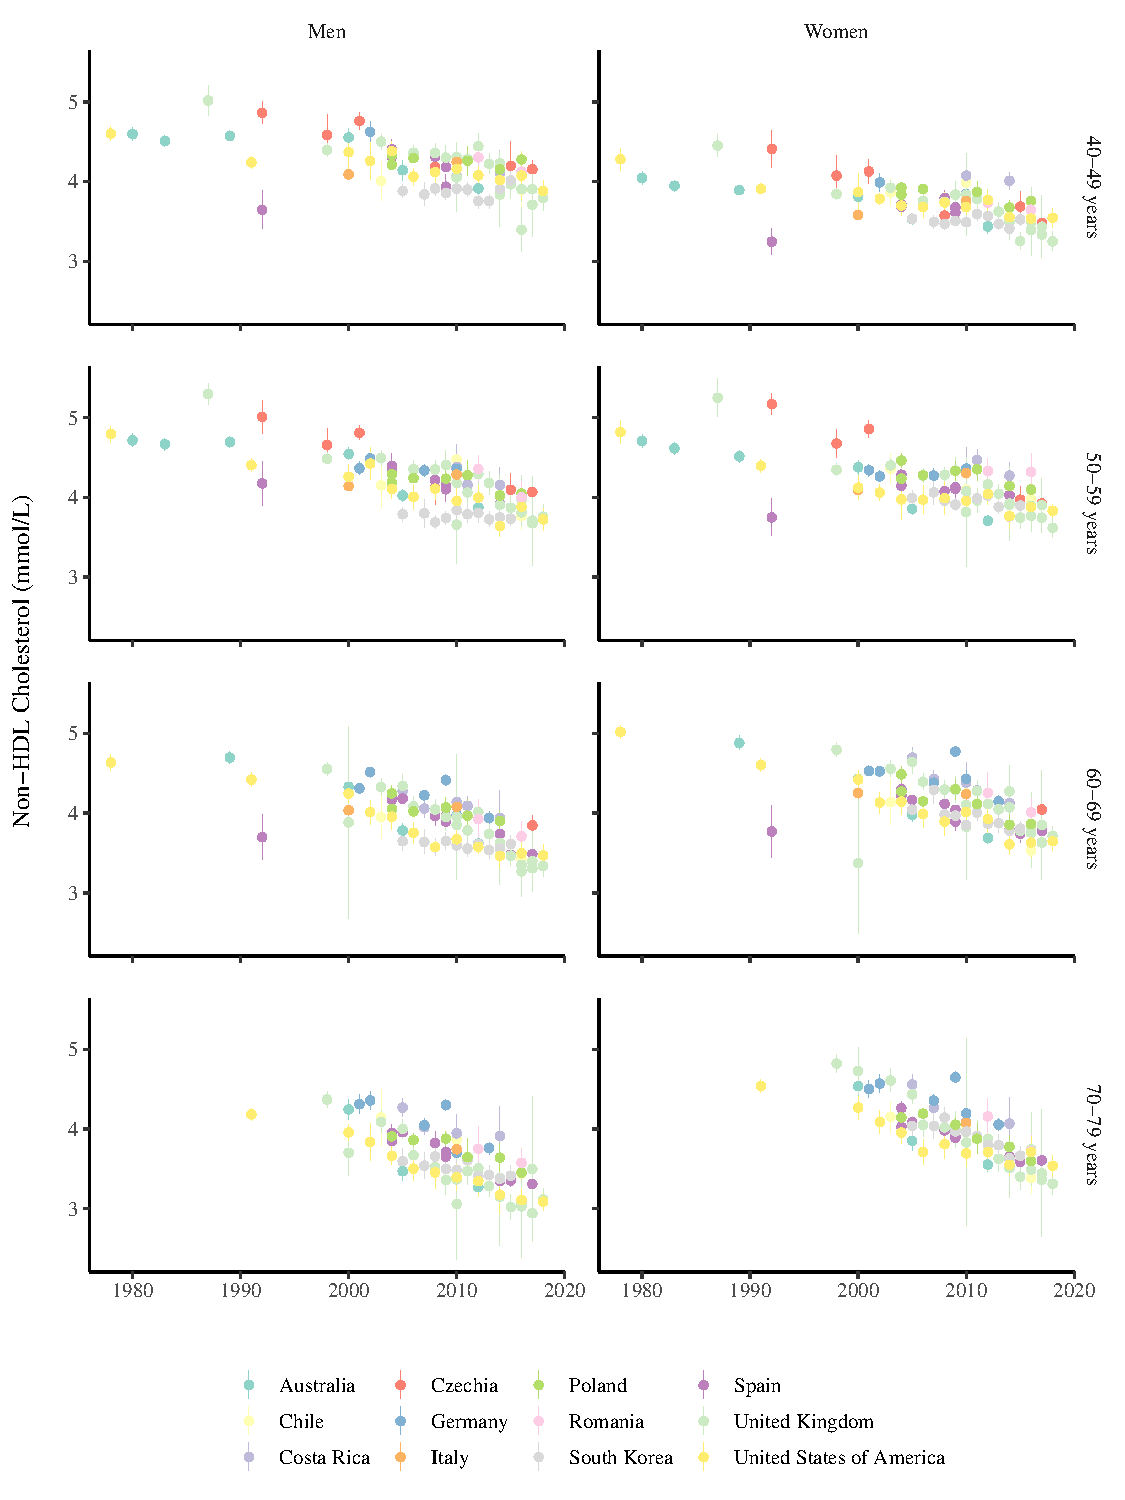
\includegraphics[width=\textwidth]{../3_figures/fig1_mean_chol.pdf}
%  \caption{Trends in mean non-HDL serum cholesterol level, by country, sex, and age group.}
%  \label{fig:mean_chol}
% \end{figure}
\begin{landscape}

    \begin{figure}[p]
        \centering
        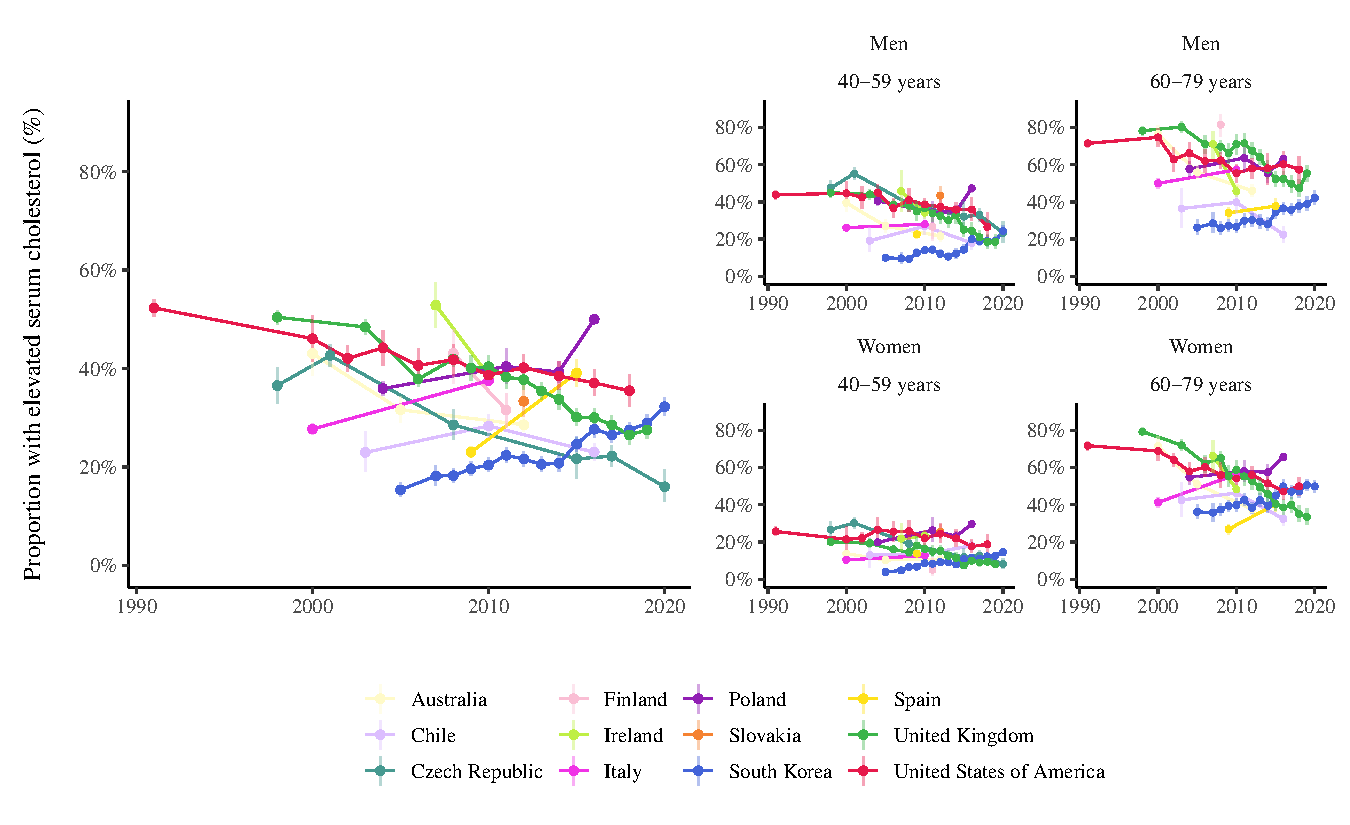
\includegraphics{../3_figures/eligible.pdf}
        \caption{Trends in elevated serum cholesterol by country and age group.}
        \label{fig:eligible}
    \end{figure}

    \begin{figure}[p]
        \centering
        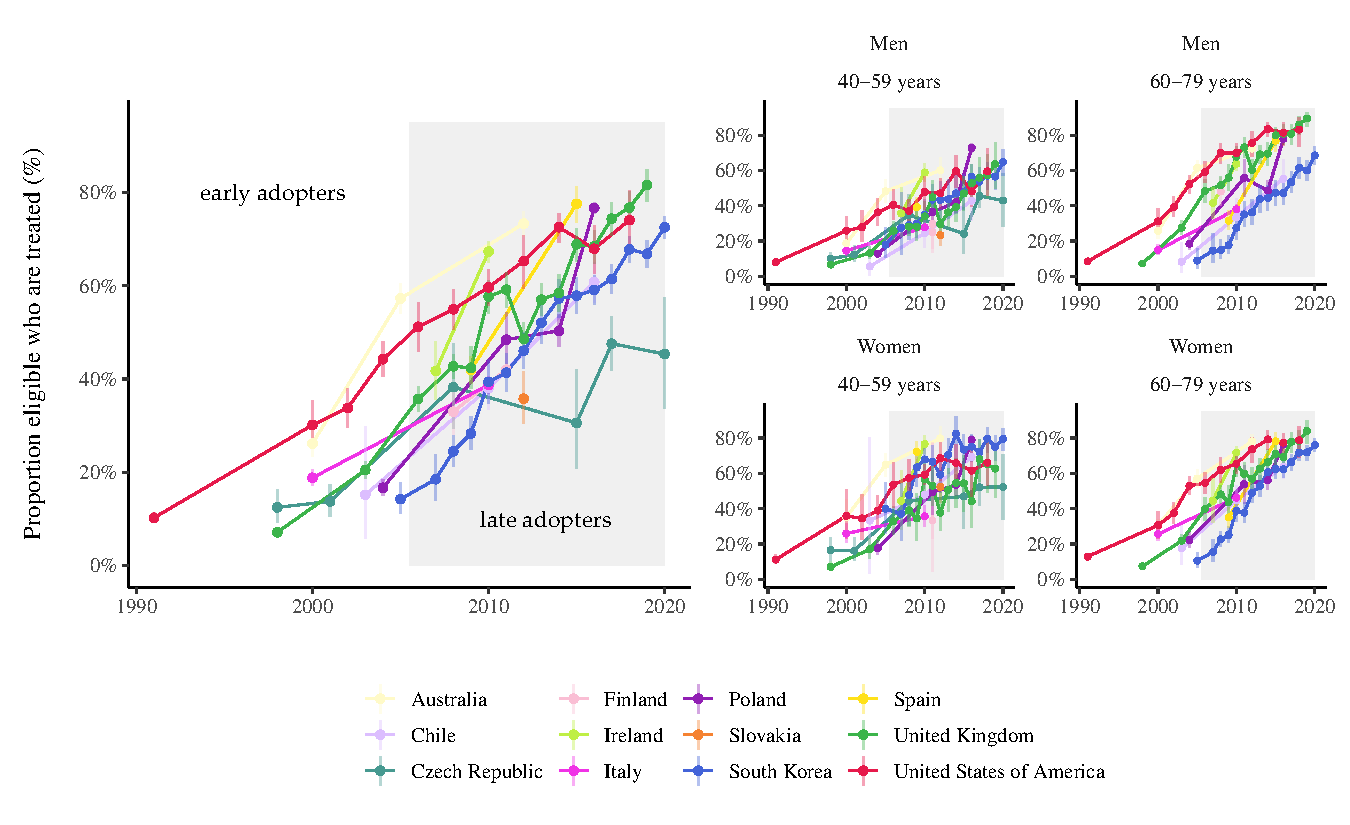
\includegraphics{../3_figures/treated.pdf}
        \caption{Trends in cholesterol treatment among participants with elevated serum cholesterol, by country and age group.}
        \label{fig:treated}
    \end{figure}

    \begin{figure}[p]
        \centering
        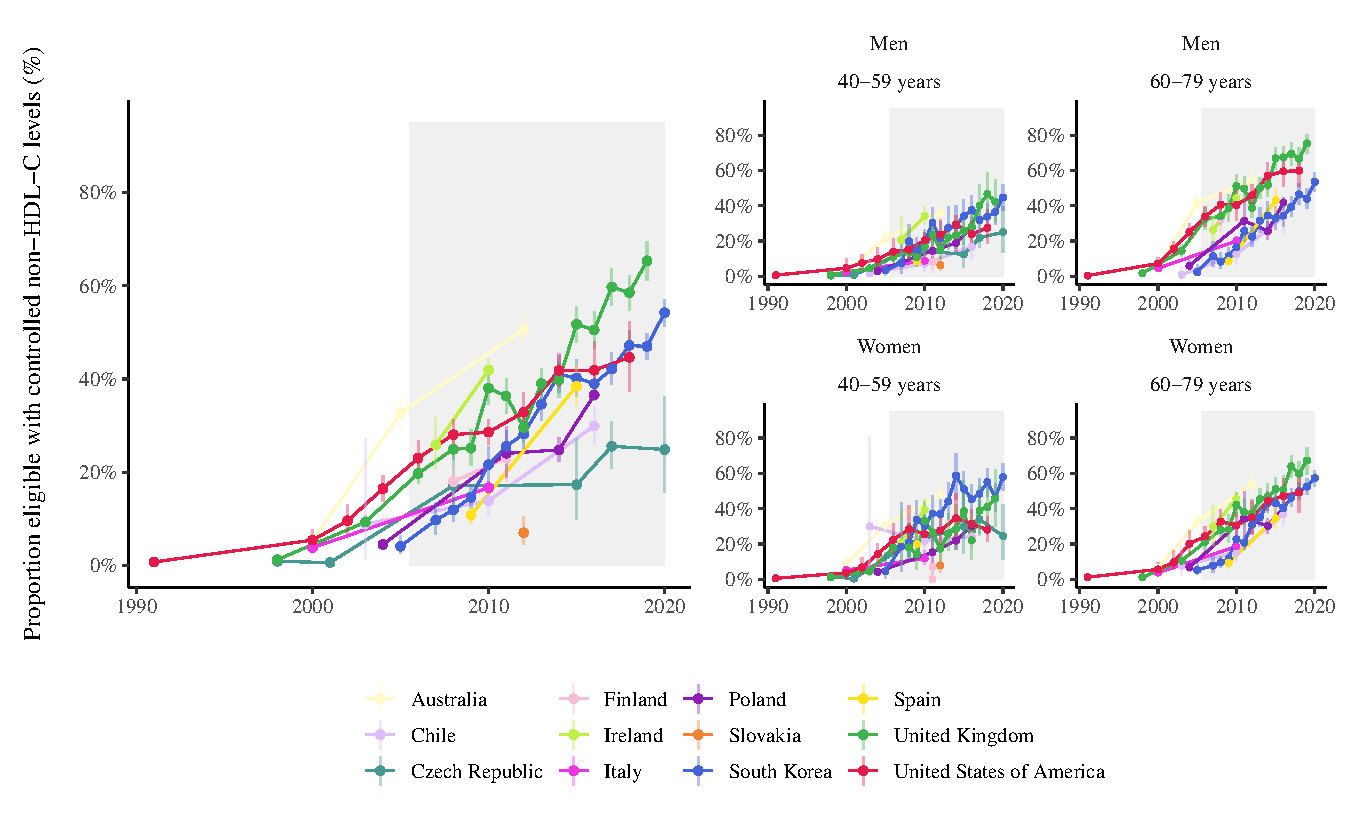
\includegraphics{../3_figures/controlled.pdf}
        \caption{Trends in controlled serum cholesterol levels among participants with elevated serum cholesterol, by country and age group.}
        \label{fig:uncontrolled}
    \end{figure}
\end{landscape}

\begin{figure}[p]
    \centering
    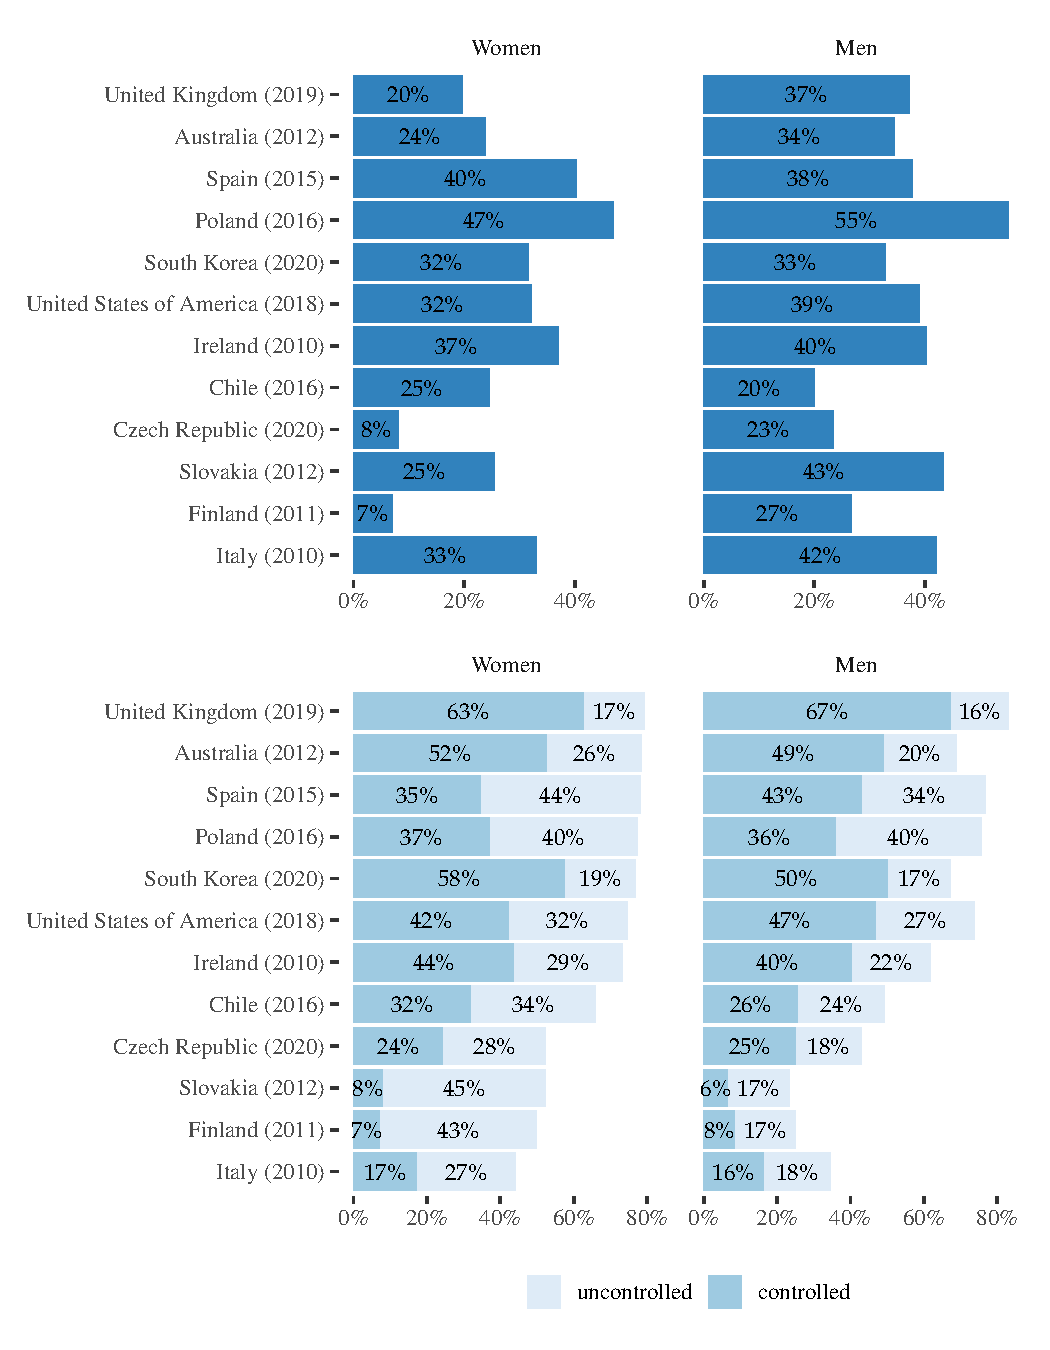
\includegraphics[width=\textwidth]{../3_figures/recent.pdf}
    \caption{Prevalence of elevated serum cholesterol and treatment and control rates in women and men aged 40 - 79 years from most recent survey.}
    \label{fig:recent}
\end{figure}

\begin{landscape}
    \begin{figure}[p]
        \centering
        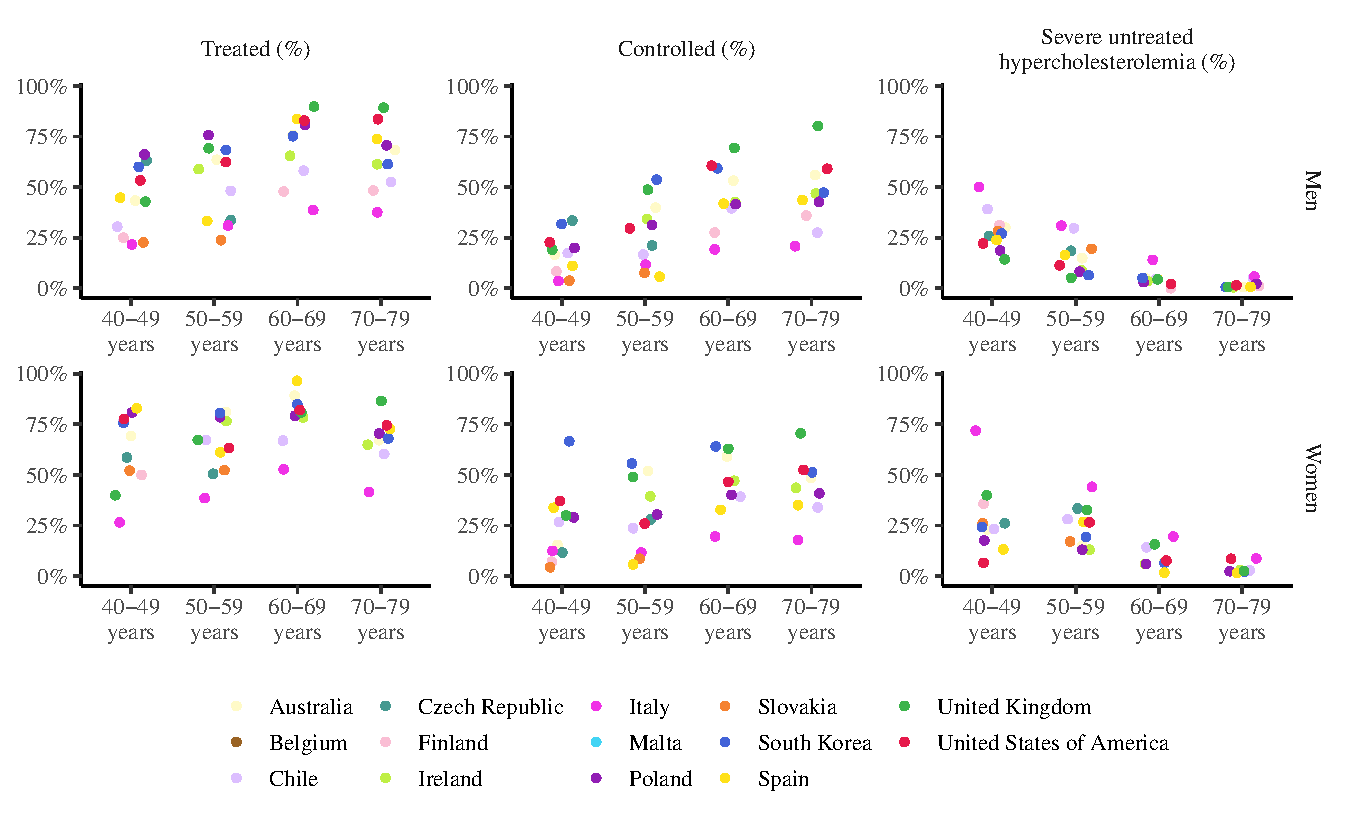
\includegraphics{../3_figures/age_gaps.pdf}
        \caption{Gaps in treatment and control of serum cholesterol in recent surveys by age.}
        \label{fig:gaps}
    \end{figure}
\end{landscape}

% \begin{figure}[hp]
%     \centering
%     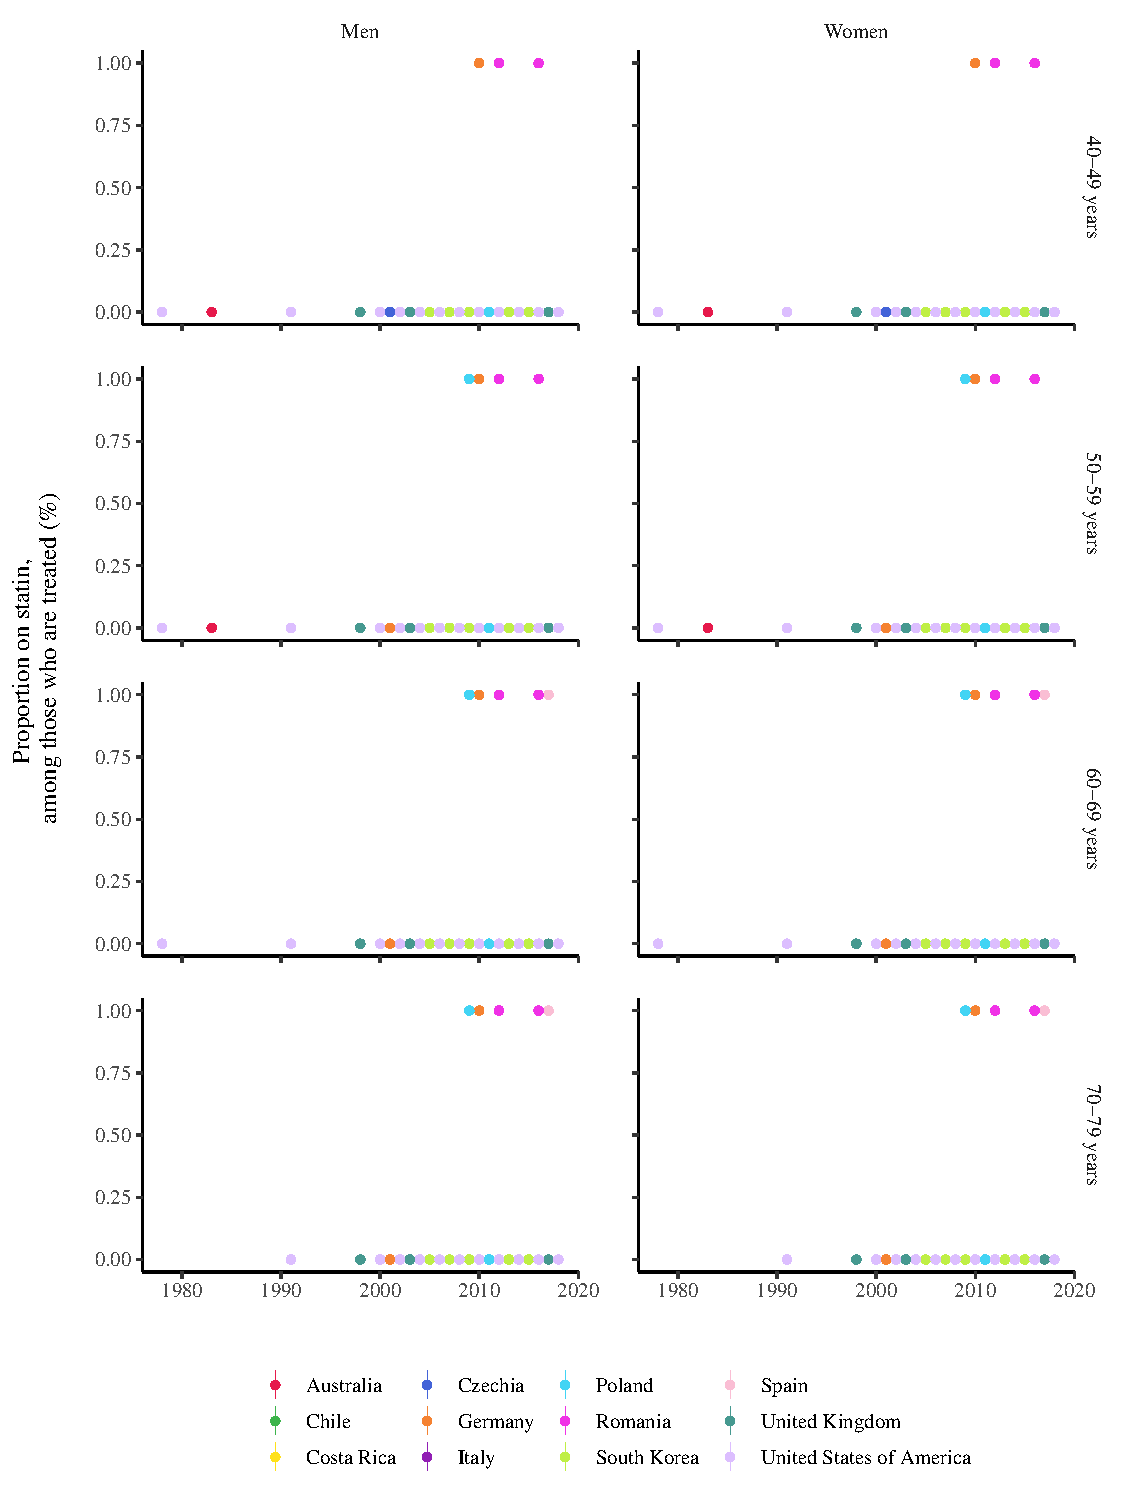
\includegraphics[width=\textwidth]{../3_figures/fig6_statin.pdf}
%     \caption{Trends in statin use among those on treatment, by country, sex, and age group.}
%     \label{fig:statin}
% \end{figure}

\clearpage 

% \section*{Research in context}

% \subsection*{Evidence before this study}
% We searched MEDLINE (via PubMed) for articles published from inception to Jun 2, 2022, using the search terms ((hypertension[Title] AND (((medication OR treatment) AND control) OR aware*) AND “blood pressure”) OR (cardiovascular[Title] AND risk factor*[Title] AND “blood pressure” AND (((medication OR treatment) AND control) OR aware*))) AND (trend* OR global OR worldwide) NOT patient*[Title]. No language restrictions were applied. We found some studies on trends in hypertension prevalence, awareness, treatment, and control in individual countries. Only three of these studies, in the USA and South Korea, used post-2010 data and reported a plateau in hypertension treatment and control. We found a few studies or reviews that compared hypertension awareness, treatment, and control across countries at one point in time, mostly using data collected from the 1980s to the 2000s. These studies mostly compared high-income countries as a group with low-income and middle-income countries, and they did not assess change over time. One study reported change in hypertension prevalence, awareness, treatment, and control in 21 countries using subnational data from the MONICA Project between two points in time (late 1980s and early 1990s). Another study, a systematic review of published studies, reported hypertension prevalence, awareness, treatment, and control in two points in time (2000 and 2010). Both of these studies did not examine trends over time in detail and did not use data collected after 2010. To our knowledge, there are no comparative studies of long-term and recent trends in hypertension awareness, treatment, and control in high-income countries.

% \subsection*{Added value of this study}
% This study provides the most comprehensive analysis of trends in hypertension awareness, treatment, and control in high-income countries using national surveys. By covering a substantially longer time period than previous studies, we noted not only substantial improvements in hypertension awareness, treatment, and control since hypertension treatment was incorporated in clinical guidelines, but also variations in the uptake of treatment and success of control across countries. By use of up-to-date national surveys in each country, we could evaluate recent trends, which revealed a plateau of the improvements in hypertension treatment coverage and control in most countries.

% \subsection*{Implications of all the available evidence}
% There has been substantial improvement in hypertension awareness, treatment, and control in high-income countries since the 1980s and 1990s, most of which was achieved in the late 1990s and early 2000s. Canada, Germany, South Korea, and the USA have the highest rates of awareness, treatment, and control, whereas Finland, Ireland, Japan, and Spain have the lowest. Even in the best performing countries, the rates fall short of those achieved in high-quality hypertension programmes—eg, the Kaiser Permanente Northern California hypertension programme. There is need for strategies that further improve the diagnosis, treatment, and control of hypertension in high-income countries.
% \clearpage 

\section*{NCD Risk Factor Collaboration (NCD-RisC)}
Christopher Boyer (Harvard TH Chan School of Public Health, USA)$^{\dagger}$; Bin Zhou (Imperial College London, UK)$^{\dagger}$; Rosie K Singleton (Imperial College London, UK); Rachel A Heap (Imperial College London, UK); Rodrigo M Carrillo-Larco (Emory University, USA); Victor Lhoste (Imperial College London, UK); Nowell H Phelps (Imperial College London, UK); Gretchen A Stevens (World Health Organization, Switzerland); Leanne M Riley (World Health Organization, Switzerland); Mária Avdičová (Banska Bystrica Regional Authority of Public Health, Slovakia)$^{*}$; Maciej Banach (Medical University of Lodz, Poland)$^{*}$; Piotr Bandosz (Medical University of Gdansk, Poland)$^{*}$; José R Banegas (Universidad Autónoma de Madrid CIBERESP, Spain)$^{*}$; Naděžda Čapková (National Institute of Public Health, Czech Republic)$^{*}$; Jerzy Chudek (Medical University of Silesia, Poland)$^{*}$; Renata Cifkova (Charles University, Czech Republic; Thomayer University Hospital, Czech Republic)$^{*}$; Juan J Cruz (Universidad Autónoma de Madrid CIBERESP, Spain)$^{*}$; Stefaan Demarest (Sciensano, Belgium)$^{*}$; Wojciech Drygas (National Institute of Cardiology, Poland; Medical University of Lodz, Poland)$^{*}$; Catterina Ferreccio (Pontificia Universidad Católica de Chile, Chile)$^{*}$; Zbigniew Gaciong (Medical University of Warsaw, Poland)$^{*}$; Simona Giampaoli (Istituto Superiore di Sanità, Italy)$^{*}$; Dušan Grafnetter (Institute for Clinical and Experimental Medicine, Czech Republic)$^{*}$; Tomasz Grodzicki (Jagiellonian University Medical College, Poland)$^{*}$; Pilar Guallar-Castillón (Universidad Autónoma de Madrid CIBERESP, Spain)$^{*}$; Jacek J Jóźwiak (University of Opole, Poland)$^{*}$; Young-Ho Khang (Seoul National University College of Medicine, Republic of Korea)$^{*}$; Urho M Kujala (University of Jyväskylä, Finland)$^{*}$; Pawel Kurjata (National Institute of Cardiology, Poland)$^{*}$; Vera Lanska (Institute for Clinical and Experimental Medicine, Czech Republic)$^{*}$; Terho Lehtimäki (Tampere University Hospital, Finland; Tampere University, Finland)$^{*}$; Esther Lopez-Garcia (Universidad Autónoma de Madrid CIBERESP, Spain)$^{*}$; Michala Lustigová (Charles University, Czech Republic; National Institute of Public Health, Czech Republic)$^{*}$; Dianna J Magliano (Baker Heart and Diabetes Institute, Australia)$^{*}$; Paula Margozzini (Pontificia Universidad Católica de Chile, Chile)$^{*}$; Karen Morgan (Royal College of Surgeons in Ireland, Ireland)$^{*}$; Malgorzata Mossakowska (International Institute of Molecular and Cell Biology, Poland)$^{*}$; Jana Námešná (Banska Bystrica Regional Authority of Public Health, Slovakia)$^{*}$; Kyungwon Oh (Korea Centers for Disease Control and Prevention, Republic of Korea)$^{*}$; Suyeon Park (Korea Centers for Disease Control and Prevention, Republic of Korea)$^{*}$; Markku Peltonen (Finnish Institute for Health and Welfare, Finland)$^{*}$; Aleksandra Piwonska (National Institute of Cardiology, Poland)$^{*}$; Olli Raitakari (University of Turku, Finland)$^{*}$; Josep Redon (University of Valencia, Spain)$^{*}$; Fernando Rodríguez-Artalejo (Universidad Autónoma de Madrid CIBERESP, Spain)$^{*}$; Marcin Rutkowski (Medical University of Gdansk, Poland)$^{*}$; Jonathan E Shaw (Baker Heart and Diabetes Institute, Australia)$^{*}$; Przemysław Slusarczyk (International Institute of Molecular and Cell Biology, Poland)$^{*}$; Jakub Stokwiszewski (National Institute of Public Health - National Institute of Hygiene, Poland)$^{*}$; Gonzalo Valdivia (Pontificia Universidad Católica de Chile, Chile)$^{*}$; Johan Van der Heyden (Sciensano, Belgium)$^{*}$; Diego Vanuzzo (MONICA-FRIULI Study Group, Italy)$^{*}$; Andrzej Więcek (Medical University of Silesia, Poland)$^{*}$; Bogdan Wojtyniak (National Institute of Public Health - National Institute of Hygiene, Poland)$^{*}$; Tomasz Zdrojewski (Medical University of Gdansk, Poland)$^{*}$; Majid Ezzati (Imperial College London, UK; University of Ghana, Ghana)$^{\ddagger}$; Goodarz Danaei (Harvard TH Chan School of Public Health, USA)$^{\ddagger}$

$^{\dagger}$ joint first authors; $^{\ddagger}$ joint senior authors; $^{*}$ contributed equally


\clearpage
\end{refsection}
\printbibliography[section=1,resetnumbers=true]

\subfile{supplement.tex}

\end{document}